To answer this question, we propose an SLA guided, security-aware continuous data provision and integration approach performed within a multi-cloud service oriented environment  (see
Figure~\ref{fig:arch}). 
We present a step-by-step data integration process and the implied  SLA categories.

In our context, data are provided by services deployed on different clouds. 
In the example of the MOOC system presented above, several producers will supply equivalent content for a given period of time. 
They will be chosen with respect to the  preferences expressed by a consumer. 

Consumers will specify queries as Datalog- or SQL-like programs including spatio-temporal attributes and preferences.
For instance, the following query $Q_1$: ``\textit{List of English poetry content providers that can provide commented Emily Dickinson poems that are close to my city and are labeled as experts, where the total cost is less than 1 dollar, using only services that preserve their anonymity}''. 

The Abstract Inter-Cloud Layer (ICL) delivers the results to the  query. 
The ICL  first identifies a set of abstract functionalities  and associated services that fit the  query. These descriptions are stored in a service description registry.

Assume that there are four content providers on English poetry that can be queried individually and two hubs that collect information from other sources like social network groups and hash tags.
Hubs  store content about given topics on  English poetry, available from particular producers (e.g., participants of a given course).
We represent these providers respectively by { e$_1$ - e$_4$}, {h$_1$}, {h$_2$}. 
We suppose that hubs  have the same interface as individual service providers.
We also suppose the existence of two free location services exporting the following interface: {loc(IP) $\rightarrow$ $\langle$ X, Y$\rangle$}, meaning that given an IP address it returns a geographic position.
All these services can potentially be combined for answering queries. Each combination will answer the query and fulfill in a specific degree the QoS requirements of the query.


%shows the general architecture of an SLA guided data integration system. 
%It accesses data services which are data providers deployed in a cloud  that provide agreed SLA's. 
%The whole process is monitored to determine whether a computed SLA is being honoured while a query is evaluated. 

%These descriptions are stored in a directory together with meta-data about the way queries are evaluated for producing results. 
%The system uses this information  by query processing and monitoring modules for rewriting queries according to given quality of service (QoS) preferences expressed by a data consumer, for example a user.The following lines describe how this query is evaluated according to our approach. 

\begin{figure*}
\center{
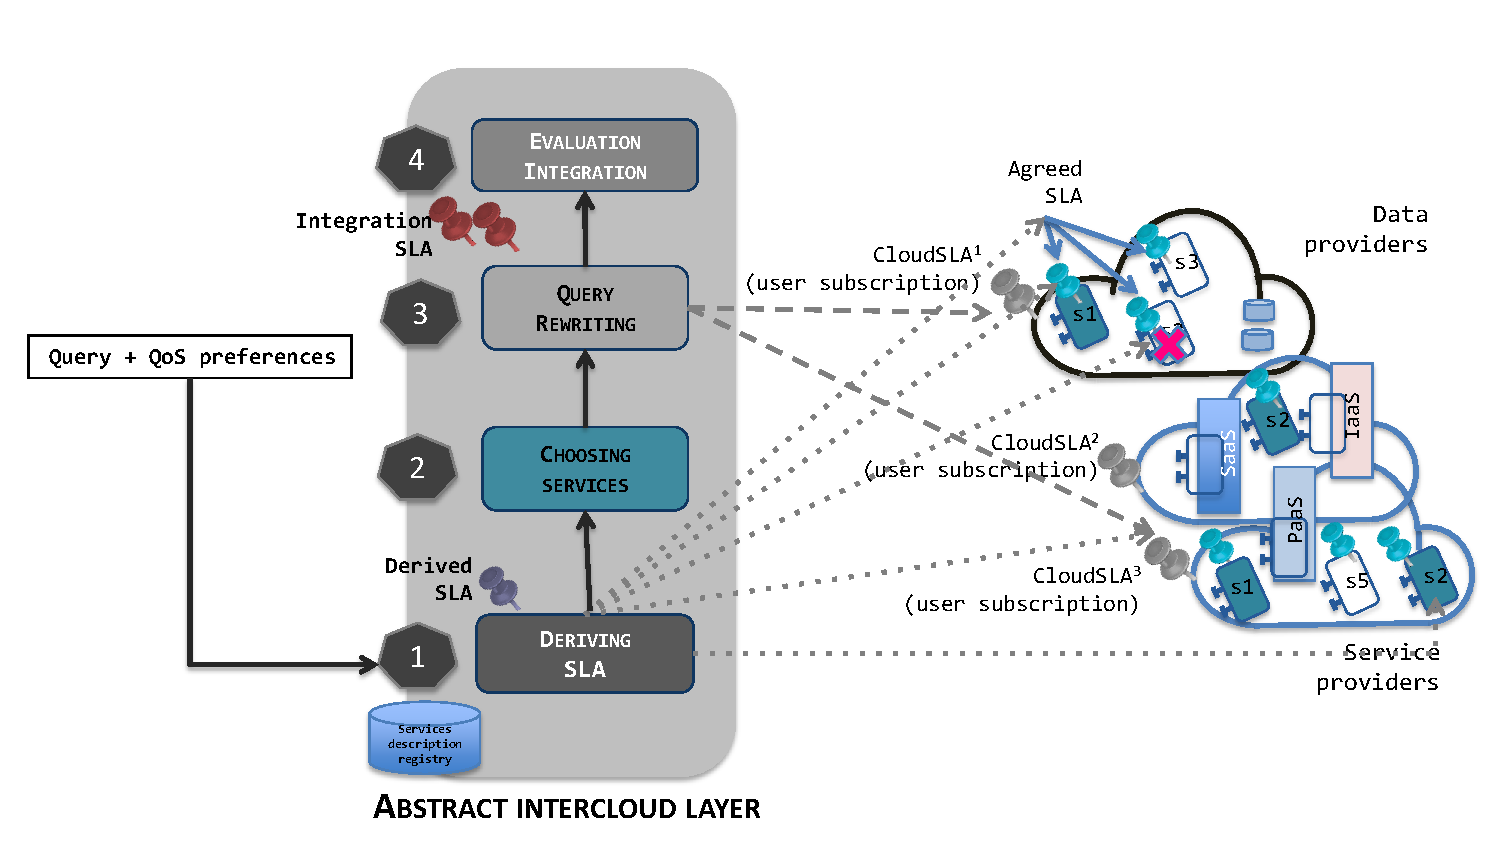
\includegraphics[width=0.65\textwidth]{workflow.pdf}
\caption{SLA guided  data integration workflow.\label{fig:arch}}}
\end{figure*}

%In order to illustrate our approach, consider a massive open online course system (MOOC) that aims at being privacy respectful of the students participating in courses and produce and consume content according to the geographic area and expertise of participants. 
%Producers are characterized according to their location, the type and topic of the content that they can provide, the access conditions (e.g. cost, inscription, or exchange unit), and the time window in which they can produce contents. 
%Consumers are described by their location, their interests requirements during a certain interval of time, the maximum total cost they are ready to pay, or the resources they are ready to provide in order to get the service, and quality of service requirements such as availability and how critical it is to consume a given type of content. 
%An energy exchange market is established in order to continuously trade  content provision/consumption ensuring that all consumers will have the content they require at every moment.

Each deployed service exports an \textit{agreed SLA} that specifies the economic cost per call, the maximum number of calls that can be done per day, the availability of the service, the average response time when a method is called, the reliability, the privacy of the produced data (whether they can be stored or not), the precision, freshness and provenance of the produced data, as defined below:

%NOTE: Agreed SLA are client-provider slas... --MARTIN

\begin{trivlist}\sf\footnotesize
\item[~-~agreedSLA$_i$:] $\langle$cost, availability, freshness, provenance, data access control, certified reputation level, location, duration$\rangle$. 
 \end{trivlist}
 
Some of these measures ({cost/call, maxCall/day}) are static and explicitly specified by the service provider. 
In contrast, the other measures should be computed by monitoring the conversations between the service and the applications that contact it.  It is the case of service reputation that will determine the way personal user data will be anonymized (Constraint1).  Some measures will be instantiated depending on the context of  the service invoked within a multi-cloud environment. It is the case for constraint 2 expressed above:   user data access credentials should be calculated according to the policies adopted by the clouds  hosting  data services.
An \textit{agreed SLA} is given as an  XML document using the specification WSLA (Web service level agreement\footnote{\footnotesize http://www.research.ibm.com/people/a/akeller/\-Data/WSLASpecV1-20030128.pdf}).

In our scenario, an example of computed measure is the cost of retrieving ``expert'' Emily Dickinson poems providers within a region, with their cost. 
The cost is determined by the  cost of the calls. 
This request  includes the price of calling a service (e.g.,  between \$0,25 - 0,50, depending on the data service), plus the price of data transmission (amount of transmitted MB through the network), the type of subscription of the user for using the network and also the cost of applying encryption algorithms if required. 
The second computed measure is service reputation that is calculated according to the feedback obtained when application contacts the service.


As aforementioned, an \textit{a-priori} SLA enforcement mechanism is mandatory to assess data integration feasibility.
To this end, non-functional characteristics of the content provision services ({i.e e$_1$-e$_4$}) are calculated by specific cloud services that enforce SLA and which should export  an API, composed of the following methods:

 
\begin{trivlist}\sf\footnotesize
\item[~-~]estim-cost$_i$(contents, req\_size, cost, prov\_size, loc), 
%QoS preferences$_\mathit{user}$, -- These should be in the query... not in the concrete services specification.
agreedSLA$_i$.

\item[~-~]engage$_i$(contents, req\_size, payment), agreedSLA$_i$.
\end{trivlist}

 

%Given user expressed QoS preferences ({QoS preferences}$_\mathit{user}$) and {agreedSLA}$_i$, 
The first method allows to obtain for each service $e_i$ the estimation of the budget (in our example, of a given course (content)) and a required minimum size. In other words, it  returns the cost of the data, as well as its  size and location.
The second method is used to engage to a data service (in our example a content data service) and will be used  if the service is retained for a composition to answer the query.

 
%The user will ask for a given derived SLA to which the provider may agree.

The ICL  obtains the set of potential services that satisfy both user preferences and   \textit{agreed SLAs} associated to services. 
For instance, the query $Q_1$ has two parts: the one that corresponds to the content required by the user  that will be solved by combining data services and the \textit{user preferences}, given by {QoS preferences}$_\mathit{user}$:
\begin{trivlist}\sf\footnotesize
\item[~-~QoS preferences$_\mathit{user}$: ] $\langle$cost, freshness, provenance, location, duration, privacy-preserving$\rangle$. 
\end{trivlist}


Let us suppose that for $Q_1$  the user is ready to pay a total cost of maximum  \$1; she requests that content providers be certified as experts (provenance) even if their data are not fresh; she requires to receive content  during  one week. Besides, she wishes to keep the content exchange private and she wants to order services by reputation. The maximum total cost will condition also the kind of privacy preserving algorithms that will be applied.
 
\begin{trivlist}\sf\footnotesize
\item[~-~QoS preferences$_\mathit{user}$: ] $\langle$cost $\leq$ \$1, freshness = ``any'', provenance = ``certified'', location = ``close'', duration = 7 days, privacy-preserving=``reputation-based''$\rangle$. 
\end{trivlist}



Cloud providers also define their SLA contracts that specify the cost per request ({cost/request}), the volume of data that can be exchanged per month ({I/0 volume/month}), the cost of transferring data or applications within the same data center or across other data centers ({datatransferCost/region}), the storage space ({storageSpace}). For example, some cloud providers let the customer  choose the geographical zone to install PaaS services and deploy applications (e.g. zone 1 is Europe). If the customer wishes to deploy services in zone 1 but store data in zone 2 the transfer cost will change.

\begin{trivlist}\sf\footnotesize
 \item[~-~cloudSLA:]  $\langle$cost/request, I/0 volume/month, datatransferCost/region, storageSpace$\rangle$.
 \end{trivlist}
 
Illustration inspired in the lowest contract provided by Azure\footnote{Azure is a trademark of Microsoft Corporation.}: 
 \begin{trivlist}\sf\footnotesize
\item[~-~cloudSLA:]  $\langle$0,05 cents per call, 8 GB I/0 volume/month, free, 1 GB storage$\rangle$. 
\end{trivlist}


 
%A content request is expressed as a query that specifies contents about a given topic with QoS preferences, independently of the possible providers. 


The next step supervised by the ICL consists in elaborating a set of potential composition specifications via a query rewriting process. Given the user query, specified as a set of abstract operations and the available services, specified in the same way, we use a Local-as-View approach~\cite{CostaAMR13} to obtain a combination of services that match the query specification.
The algorithm in~\cite{CostaAMR13} is being modified to deal with agreedSLA and QoS user preferences.

 

In this paper, we are interested in the process of rewriting queries  considering QoS user preferences and SLAs.
This process includes the following phases: 
\begin{trivlist}
\item[~1)]  User preferences (including cloud SLA according to user subscriptions) and \textit{agreed SLA} are  used to produce a \textit{derived SLA} to be associated to the query. 
{\em Derived SLA}  influences the choice of services that will be used to build the result; 
\item[~2)] Computing service compositions that rewrite the initial query and that are used to  build query results. 
The \textit{agreed SLA} exported by the chosen services is added as conditions in  each re-written query expression. 
Rewritten queries expressed as service composition can fully or partially comply with the \textit{derived SLA}.  An \textit{integration SLA} is  computed for guiding  negotiation (in the case of partial compliance)  and the implementation of the final integration; 
\item[~3)]   Integration process guided by the \textit{integration SLA}.
\end{trivlist}
 


